\documentclass[a4paper,11pt]{article}
\usepackage{amsmath,amsthm,amsfonts,amssymb,amscd,amstext,vmargin,graphics,graphicx,tabularx,multicol} 
\usepackage[francais]{babel}
\usepackage[utf8]{inputenc}  
\usepackage[T1]{fontenc} 
\usepackage{pstricks-add,tikz,tkz-tab,variations}
\usepackage[autolanguage,np]{numprint} 

\setmarginsrb{1.5cm}{0.5cm}{1cm}{0.5cm}{0cm}{0cm}{0cm}{0cm} %Gauche, haut, droite, haut
\newcounter{numexo}
\newcommand{\exo}[1]{\stepcounter{numexo}\noindent{\bf Exercice~\thenumexo} : \marginpar{\hfill /#1}}
\reversemarginpar


\newcounter{enumtabi}
\newcounter{enumtaba}
\newcommand{\q}{\stepcounter{enumtabi} \theenumtabi.  }
\newcommand{\qa}{\stepcounter{enumtaba} (\alph{enumtaba}) }
\newcommand{\initq}{\setcounter{enumtabi}{0}}
\newcommand{\initqa}{\setcounter{enumtaba}{0}}

\newcommand{\be}{\begin{enumerate}}
\newcommand{\ee}{\end{enumerate}}
\newcommand{\bi}{\begin{itemize}}
\newcommand{\ei}{\end{itemize}}
\newcommand{\bp}{\begin{pspicture*}}
\newcommand{\ep}{\end{pspicture*}}
\newcommand{\bt}{\begin{tabular}}
\newcommand{\et}{\end{tabular}}
\renewcommand{\tabularxcolumn}[1]{>{\centering}m{#1}} %(colonne m{} centrée, au lieu de p par défault) 
\newcommand{\tnl}{\tabularnewline}

\newcommand{\bmul}[1]{\begin{multicols}{#1}}
\newcommand{\emul}{\end{multicols}}

\newcommand{\trait}{\noindent \rule{\linewidth}{0.2mm}}
\newcommand{\hs}[1]{\hspace{#1}}
\newcommand{\vs}[1]{\vspace{#1}}

\newcommand{\N}{\mathbb{N}}
\newcommand{\Z}{\mathbb{Z}}
\newcommand{\R}{\mathbb{R}}
\newcommand{\C}{\mathbb{C}}
\newcommand{\Dcal}{\mathcal{D}}
\newcommand{\Ccal}{\mathcal{C}}
\newcommand{\mc}{\mathcal}

\newcommand{\vect}[1]{\overrightarrow{#1}}
\newcommand{\ds}{\displaystyle}
\newcommand{\eq}{\quad \Leftrightarrow \quad}
\newcommand{\vecti}{\vec{\imath}}
\newcommand{\vectj}{\vec{\jmath}}
\newcommand{\Oij}{(O;\vec{\imath}, \vec{\jmath})}
\newcommand{\OIJ}{(O;I,J)}


\newcommand{\reponse}[1][1]{%
\multido{}{#1}{\makebox[\linewidth]{\rule[0pt]{0pt}{20pt}\dotfill}
}}

\newcommand{\titre}[5] 
% #1: titre #2: haut gauche #3: bas gauche #4: haut droite #5: bas droite
{
\noindent #2 \hfill #4 \\
#3 \hfill #5

\vspace{-1.6cm}

\begin{center}\rule{6cm}{0.5mm}\end{center}
\vspace{0.2cm}
\begin{center}{\large{\textbf{#1}}}\end{center}
\begin{center}\rule{6cm}{0.5mm}\end{center}
}



\begin{document}
\pagestyle{empty}


\begin{center}
\textbf{ {\large TP 1  : Arithmétique}}
\end{center}

\vspace*{0.5cm}

\exo{} 

\q Trouver un nombre à quatre chiffres : 
\bi
\item divisible par 2; 
\item non divisible par 9;
\item divisible par 3;
\item divisible par 5.\\

\ei

\q Parmi les cinq nombres suivants, un seul n'est pas premier. Lequel ? \\
43 ; 53 ; 63 ; 73 ; 83. \\

\vspace*{0.5cm}

\exo{} \textbf{Les nombres amicaux}\\
Deux nombres sont \textbf{amicaux} quand chacun est égal à la somme des diviseurs de l'autre (excepté le nombre).\\

Lister les diviseurs de 220 et 284 et dire s'ils sont amicaux ou non.\\


\vspace*{0.5cm}



\exo{}\textbf{Les nombres gentils}\\
Un nombre est \textbf{gentil} s'il est multiple des dix premiers nombres entiers.\\

\initq \noindent \q Expliquer pourquoi 10 080 est gentil. \\
\q Trouver le plus petit nombre gentil, en expliquant votre recherche.\\ 

\vspace*{0.5cm}

\exo{}

L'ensemble des écrits de Victor Hugo a été republié après sa mort en 53 volumes. La bibliothécaire classe ces volumes à raison de 8 volumes par étagères.\\

\noindent \initq \q Combien d'étagères faut-il pour exposer toute l'\oe{uvre} de Victor Hugo?\\
\q Combien de volumes l'étagère incomplète contiendra-t-elle?\\
\vspace*{0.5cm}


\exo{}

Le numéro INSEE ,ou numéro de sécurité sociale, est un numéro composé de 13 chiffres permettant d'identifier chaque personne en France.\\
Pour limiter les erreurs de saisie, le numéro INSEE est suivi d'un nombre appelé clé de contrôle. Cette clé est la différence entre 97 et le reste de division euclidienne du numéro INSEE par 97.\\

\noindent \initq \q Quelle est la clé du numéro INSEE suivant ?
\begin{center}
\includegraphics[scale=0.4]{INSEE.eps} 
\end{center}

\q Un site refuse le numéro : 2 75 02 87 085 078 11. Expliquer pourquoi.\\


\vspace*{0.5cm}

\exo{} 
Le centurion est fier de son armée. Pour le défilé à Rome, il demande à ses soldats de se ranger par lignes de cinq, mais il reste quatre soldats.\\
Il leur demande alors de se ranger par lignes de six, mais il reste cinq soldats.\\
Il leur demande de se ranger par lignes de huit, mais il reste sept soldats.\\

\noindent \initq \q Combien cette armée comporte-t-elle de soldats sachant qu'elle compte moins de deux-cents hommes ?\\
\q Par lignes de combien de soldats ce centurion pourra-t-il ranger correctement son armée ?\\






\end{document}
